\documentclass[11pt]{article}

\usepackage[font=footnotesize]{caption}
\usepackage{float}
\usepackage{epsf}
\usepackage{epsfig}
\usepackage{subfigure}
\usepackage{latexsym}
\usepackage{booktabs}
\usepackage{graphicx}
\usepackage[table,xcdraw]{xcolor}
\usepackage{color, colortbl}
\usepackage{wrapfig}
\usepackage{multirow}
\usepackage{tabularx}
\usepackage{hyperref}
\usepackage{xcolor}
\usepackage{mdwlist}
\usepackage{pdfpages} 
\usepackage{tabto}  



\usepackage{amsmath, amsfonts, amssymb}
\usepackage[hmargin=1in,vmargin=1.2in]{geometry}
\usepackage{url}
\usepackage{multirow}
\usepackage[bottom]{footmisc}
\usepackage{afterpage}
\usepackage{eurosym}
\usepackage{enumitem}
\usepackage{soul}
% *******************************************
\usepackage{lineno}
\usepackage{setspace}
% *******************************************

\interfootnotelinepenalty=80 
\floatingpenalty=0\relax
\widowpenalty=1000
\clubpenalty=1000


\def\proj{{\textbf{FRESNEL\ }}}
\def\proje{{\textbf{FRESNEL}}}
\def\met{{\textbf{METEOR\ }}}
\def\mete{{\textbf{METEOR}}}
\def\naz{{Nazar\'{e}\ }}
\def\naze{{Nazar\'{e}}}

\setlength{\parskip}{0pt}
\setlength{\parsep}{0pt}
\setlength{\headsep}{0pt}
\setlength{\topskip}{0pt}
\setlength{\topmargin}{0pt}
\setlength{\topsep}{0pt}
\setlength{\partopsep}{0pt}

\newtheorem{definition}{Definition}
\newcommand{\hide}[1]{}
\newcommand{\kcomment}[1]{{\color{red}{KR: #1}}}
\newcommand{\rmcomment}[1]{{\color{blue}{RM: #1}}}
\newcommand{\com}[1]{{\color{blue}{#1}}}
\newcommand{\hcom}[1]{{\color{white}{#1}}}
\newcommand{\lc}[1]{\textcolor{blue}{#1}}

\newcounter{quotenumber}

% \newenvironment{numquote}{%
%     \begin{enumerate}%
%      \setcounter{enumi}{\value{quotenumber}}%
%      \color{darkgray}
%     \item \begin{quote}%
% }{%
%     \end{quote}%
%     \setcounter{quotenumber}{\value{enumi}}
%     \end{enumerate}%
% }%

% \makeatletter
% \def\myitem{%
%    \@ifnextchar[ \@myitem{\@noitemargtrue\@myitem[\@itemlabel]}}
% \def\@myitem[#1]{\item[#1]\mbox{}}
% \makeatother



% \newcommand\blankpage{%
%     \null
%     \thispagestyle{empty}%
%     \addtocounter{page}{-1}%
%     \newpage}

\setcounter{secnumdepth}{1} 

\let\oldthebibliography\thebibliography
\let\endoldthebibliography\endthebibliography
\renewenvironment{thebibliography}[1]{
  \begin{oldthebibliography}{#1}
    \setlength{\itemsep}{0em}
    \setlength{\parskip}{0em}
}
{
  \end{oldthebibliography}
}
% \linespread{0.98}
\parskip 0.1cm


\title{On Model-Driven Ocean Exploration}

\author{
Renato Mendes\textsuperscript{1,2,3,*},
Lucrezia Bernacchi \textsuperscript{1},
Leonardo Azevedo \textsuperscript{},
Ana F. Duarte \textsuperscript{},\\
Marina Cunha \textsuperscript{},
Clara Rodriguez \textsuperscript{},
João Borges de Sousa \textsuperscript{2,3},
João Vitorino \textsuperscript{},\\
Ajit Subramaniam \textsuperscript{},
Kanna Rajan \textsuperscript{}
\\
\\
\textsuperscript{1}{\scriptsize +ATLANTIC CoLAB, Lisboa, Portugal}\\
\textsuperscript{2}{\scriptsize Laboratório de Sistemas e Tecnologia Subaquática (LSTS), Faculdade de Engenharia da Universidade do Porto, Portugal}\\
\textsuperscript{3}{\scriptsize Laboratório Associado de Energia, Transportes e Aeronáutica (LAETA), Porto, Portugal}\\
\textsuperscript{1}{\scriptsize Universidade de Aveiro, Portugal}\\
\textsuperscript{1}{\scriptsize Lamont-Doherty Earth Observatory, Columbia University, New York}\\
\textsuperscript{1}{\scriptsize Instituto Hidrogr{\'a}fico Lisboa, Portugal}\\
\textsuperscript{1}{\scriptsize RAND Corporation, Washington D.C \& Faculdade de Engenharia da Universidade do Porto, Portugal}\\
\textsuperscript{*}\texttt{{\scriptsize renato.mendes@colabatlantic.com}}
}
\date{} 
\begin{document}

% \setcounter{secnumdepth}{2} 
% \vspace{+0.5cm}

\maketitle
\section{Introduction}
\label{sec:intro}

The coastal ocean, the marine areaS extending from the coastline to
the continental slope, encompassing the continental shelf, constitutes
one of the most dynamic and complex regions of the ocean. These areas
are characterized by highly variable forcing mechanisms, intricate
topographies, and coastline geometries. They are forced by a wide
range of physical and biogeochemical processes which occur across
diverse spatial and temporal scales. They are among the most
productive and economically significant areas of the world’s oceans,
benefiting from terrestrial inputs via river discharges and nutrient
renewal driven by upwelling processes. As a result and in part,
coastal areas concentrate a great proportion of human maritime
activities, from fisheries and offshore aquaculture to renewable
energy exploitation. Moreover, the coastal ocean acts as an interface
between deep-ocean processes and coastal environment, modulating how
large-scale phenomena — such as climate-driven changes or extreme
weather events — impact coastal populations. It also regulates, for
example, how anthropogenic influences originating on land are
redistributed and affect marine ecosystems \cite{greene25}.

The complex interplay between physical, chemical, and biological
processes in the coastal ocean can rapidly amplify or modulate the
impacts of extreme events such as storms, flooding, or pollution
incidents. Furthermore, the coastal ocean serves as a key interface
where large-scale oceanic and atmospheric changes manifest their
consequences for coastal ecosystems. Accurately forecasting the state
of the coastal ocean is therefore essential not only for safeguarding
environmental and economic interests, but also for enhancing
resilience to climate variability, natural hazards, and human-induced
pressures.  Achieving this, however, remains a major scientific and
technological challenge, given the high variability, rapid dynamics,
and observational constraints inherent to these regions.

Ocean models have become essential tools for predicting the ocean
state and underpin a wide range of societal applications, from climate
forecasting to pollution monitoring and resource management. However,
these models are inherently imperfect representations of complex
reality. Data assimilation techniques — where observational data are
integrated into models — play a critical role in correcting or
adjusting model errors and improving their forecasting
capabilities. Yet, the success of data assimilation depends heavily on
the availability, quality, and relevance of observations.

Observations of the ocean are obtained through multiple sources.
Satellite remote sensing offers extensive spatial coverage but is
limited to surface measurements with usually low spatial resolution
and often compromised by atmospheric conditions. In situ observations,
whether from ships, moorings, or drifting platforms, provide higher
accuracy but suffer from limited spatial and temporal coverage, high
operational costs, and logistical constraints — particularly high in
coastal regions. Recent technological advances have enabled the use of
autonomous underwater vehicles (AUVs) and other robotic platforms,
offering flexible, mobile, and increasingly autonomous means of
sampling ocean properties with high spatiotemporal resolution and low
logistic footprint
\cite{das10,das11b,olaya12,graham12,jdas13,das15,sousa16,fossum18,fossum19b}.

However, even with these new tools, efficiently gathering data at the
right spatial and temporal scales remains a complex challenge. AUVs
are constrained by endurance, communication bandwidth, and operational
risks such as vessel traffic, high currents and bathymetry. In
addition, the ocean itself remains highly dynamic with key processes
often evolving faster than traditional sampling strategies can
capture. This opens the door to adaptive sampling strategies, where
observation efforts are guided by model outputs and uncertainty
estimates to maximize the relevance of collected data. Adaptive
sampling \cite{BinZhang07,Singh09,smith14,fossum19} represents a
fundamental shift: instead of executing pre-planned missions,
autonomous vehicles dynamically prioritize areas for observation.

One approach that we articulate here is combining model predictions
with adaptive AUV sampling. Doing so combines predicted model
uncertainties in comparison with prior data assimilation process with
availabe obervations. Model forecasts identify where uncertainty is
highest or where new observations are expected to have the greatest
impact in reducing forecast errors. Vehicles are then directed to
sample these areas, and their data are in turn assimilated back into
the models, generating improved forecasts for subsequent adaptive
planning as a virtuous cycle. Doing so closes a critical feedback loop
between models and observations; model prediction generates a forecast
and associated uncertainty field while adaptive sampling targets areas
of maximum predicted uncertainty. Data assimilation from these high
uncertainty regions are then incorporated into the model such that new
predictions benefit from improved in-situ data, closing the loop.
Such a \textit{data cycle} approach promises to significantly enhance
the skill of ocean forecasts, especially in the complex coastal
environment where processes occur over a wide range of scales and
where human and environmental stakes are high. It also has the
potential to improve operational efficiency by optimizing the
deployment of costly and resource-constrained observational assets. 
WE MAY WANT TO EXPLAIN THAT THIS CAN ONLY BE DONE WITH AUVS AND AT A MODERATE COST IN COMPARISON TO TRADITIONAL SAMPLING METHODS


IT MAY ALSO BE A GOOD IDEA TO HAVE A SHORT PARAGRAPH OM INNOVATION CLAIMS: something like

This has been done before, but we innovate in several aspects: 
\begin{itemize}
    \item Near-real time data visualization enable real.time response by operators..
    \item Simultaneous deployments in geographically separate subareas in the area of operations.
    \item Coordination also included risk minimizing considerations. This enabled operations in tight time intervals to collect data where it was needed taking advantage of openings provided by trawlers between consective legs.
    \item Parameterized framework enabling fine tuning of the overall approach. 
    \item Dense grid of observations.
    \item The sampling algorithm is not based only on position, but on error distributions and closed tours to maximize area coverage and utilization of the auvs.
    \end{itemize}

WHAT DO YOU THINK?

\begin{figure}[!]
  \centering
  \includegraphics[scale=0.5]{fig/ensemble-2.jpg}
  \caption{\proj demonstrates the value of integrating ocean models
    with adaptive robotic vehicles in the coastal ocean, to increase
    model skill while increasing model accuracy and prediction within
    a tight control loop.}
  \label{fig:block-diag}
\end{figure}



In this study, we address the challenge of such loop closure by
implementing and evaluating a complete data cycle — from model
prediction, to uncertainty projection, to adaptive sampling and data
assimilation — in a coastal ocean environment. The work was conducted
within the framework of \proj (\textbf{F}ield expe\textbf{R}iments for
mod\textbf{E}ling, a\textbf{S}similatio\textbf{N} and
adaptiv\textbf{E} samp\textbf{L}ing), a project specifically designed
to explore and test model-driven robotic exploration strategies. \proj
provided the experimental setting and operational assets to
demonstrate how model-based uncertainty fields can drive adaptive
sampling missions aimed at improving ocean model predictive skills to
enhance ocean forecasts in highly dynamic coastal environments
(Fig. \ref{fig:block-diag}). The experimental results obtained within
\proj serve to illustrate and validate the proposed approach,
highlighting the practical benefits and challenges of real-world
adaptive ocean exploration. Furthermore, we demonstrate that this
sampling robotic system offers unprecedented capabilities for ocean
studies by providing samples in close to real-time and enabling
scientists to adaptively re-task AUVs within minutes if some
interesting feature is detected.


%\subsection{The domain: \naze, Portugal}
\label{sec:naz}

\begin{figure}[!b]
  \vspace{-0.5cm} 
  \centering 
  \subfigure[Map of Portugal and the study area highlighted with the red
  rectangle.]{\label{fig:po-map}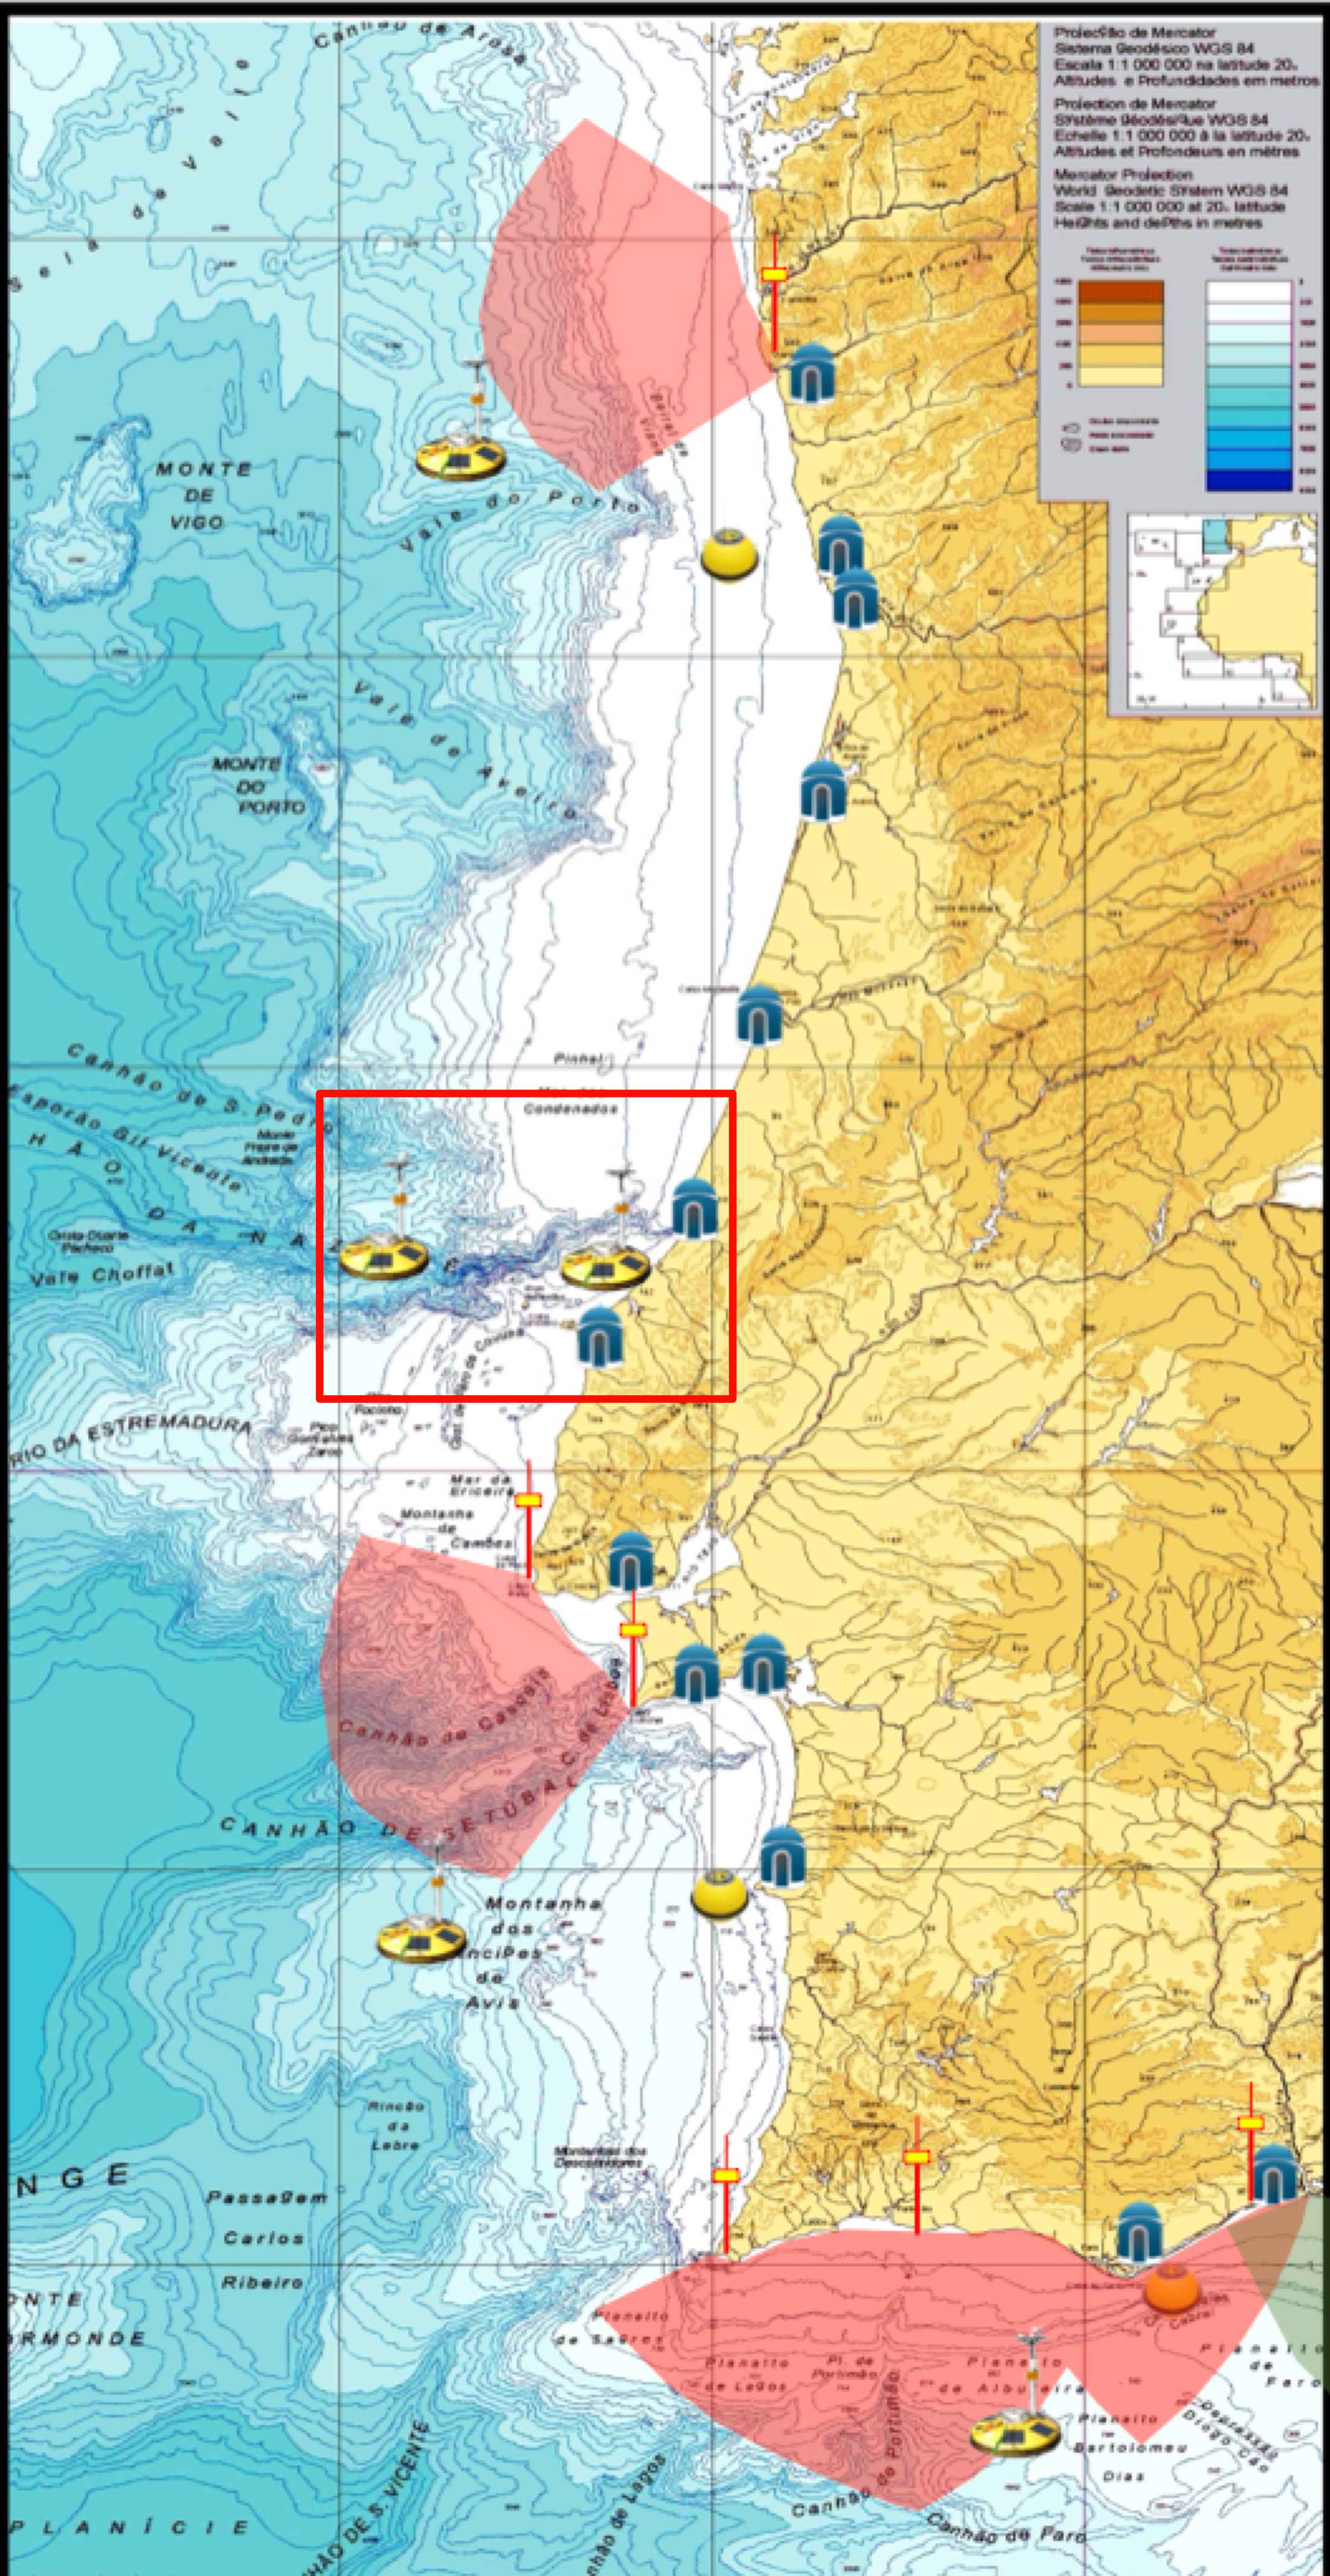
\includegraphics[scale=0.5]{fig/po-map.jpeg}}
  \hspace{+0.3cm} 
  \subfigure[Zoomed in bathymetry showing the \naz canyon-Berlengas
  area (isobaths with depth in meters) and its environment including
  the placement of the two buoys.]{\label{fig:domain}\includegraphics[scale=0.55]{fig/domain.jpg}}
  \caption{\subref{fig:po-map} \& \subref{fig:domain} show detailed
    views of the proposed study area for \proj off the coast of
    mainland Portugal. The \naz Canyon is a significant feature of
    this area and a driver for the bio-geophysics of the domain. The
    shaded blue area is the expected glider operations region which
    will inform the model about boundary conditions and off-shore
    waters being entrained into the canyon.}
  \label{fig:studyarea-1}
\end{figure}

\proj will focus on the area of influence of \naz Canyon located in
the central part of the western Portuguese coast and broadly extending
from 39.2$^{\circ}$N (south of Peniche) to 39.9$^{\circ}$N north of
\naz (Fig. \ref{fig:po-map}). This is a coastal ocean area well
exposed to the influence of the North Atlantic and marked by
important topographic features such as:

\begin{itemize}[noitemsep,topsep=0pt,parsep=0pt,partopsep=0pt]

\item important changes of the continental margin associated with the
  transition from the large Estremadura Plateau to the south, to the
  relatively narrow shelf north of \naz

\item the presence of a long and narrow submarine \naz canyon that
  extends for more than 200 km from the head, just a few hundreds of
  meters from the beach of \naze, incising the shelf into the abyssal
  area

\item the presence of island environments -– the Berlengas archipelago
  located a few tens of kilometers offshore the coast which is a
  \texttt{Natura2000} site recognized as a unique repository of
  species and habitat diversity on the western boundary of Europe. It
  was recently classified by UNESCO as a Biosphere Reserve. The
  biogeographic, geologic and oceanographic settings of this region,
  accentuated by the presence of the \naz canyon, are critical for the
  high levels of biological productivity and biodiversity, that induce
  dynamic ecological processes and support many ecosystem services

\end{itemize}


\vspace{+0.5cm}
The \naz Canyon area of influence is not directly impacted by major
riverine outflows. The main rivers influencing the western Portuguese
continental margin are the Douro (located about 170 km to the north of
\naze) and the Tagus (located at about 100 km to the south) with
smaller contributions from the Mondego (50 km to the north). During
the winter and early spring the combined influence of the Douro and
other smaller rivers such as the Mondego reach the \naz Canyon area
during periods of northerly winds and upwelling conditions, appearing
as a low salinity water plume occupying the first 30 m of the water
column and extending over the complete shelf as the result of offshore
transport associated with the prevailing upwelling conditions. The
influence of the Tagus River on the area is less clear, largely due to
the combination of the large Estremadura Plateau with the shallow
ridge between Cape Carvoeiro and Berlengas areas and associated
circulation characteristics. More expressive for the conditions in the
area is the contribution of the small riverine sources that indent the
\naze-Peniche coast during periods of important precipitation. These
include the contributions of the small Alcoa and Tornadas rivers, of a
large number of very small fresh water courses (ribeiras) or from the
Obidos Lagoon. Previous observations have showed \cite{martins10} that
these contributions combine fresh waters with high turbidity and high
nutrient content that can extend its influence over the complete
shelf.

The evolution of wind forcing and wave conditions affecting this area
is largely determined by the seasonal migration of the Azores High
Pressure System. From May to September the Azores High is typically
located at its northernmost position, offshore the Iberian
Peninsula. During this period, the western Portuguese margin is
located on the eastern branch of the High, under the influence of
persistent (upwelling favorable) northerly winds that during the
summer months, are reinforced by the establishment of a thermal low
over central Iberia. The area is also protected from the influence of
synoptic low pressure systems, showing typically low energy swells
(although affected by locally generated sea breeze
circulation). During the winter months the conditions prevailing along
the western Portuguese margin are largely associated with the phase of
the winter North Atlantic Oscillation (NAO). During the negative phase
of the winter NAO the Azores High is typically located southwest of
the Iberian Peninsula and the western Portuguese coast is under the
influence of westerly and southwesterly wind forcing that frequently
promote downwelling conditions. During those periods the area is also
exposed to the direct influence of synoptic low pressure systems and
associated highly energetic waves. During the positive phases of the
winter NAO, the Azores High remains at northward latitudes leading to
frequent periods of northerly winds and upwelling conditions along the
western Portuguese margin. During these periods the area is largely
protected from the direct influence of low pressure synoptic systems
and shows a less energetic wave regime in general, although impacted
by large swells that are generated far in the North Atlantic.

The atmospheric forcing conditions described above establish some
complex dynamics in the \naz canyon area of influence, marked by the
interactions of the shelf and slope circulation with the canyon
topography and island environments and by the manifestation of
important meso-scale features such as the upwelling filament of Cape
Carvoeiro. In addition, the rich topography of the area also promotes
complex tidal dynamics. Barotropic tidal currents along the western
Portuguese margin are in general dominated by the semidiurnal lunar
constituent (M2), within a period of 12 hours and 25 minutes.  In the
shelf north of \naz canyon the barotropic tidal current magnitudes are
dominated by the M2 constituent and show magnitudes of 5-10 cm/s. To
the south of Peniche, the large and shallow Estremadura Plateau
constitutes an area of intensification of the barotropic tidal
currents, both for the dominant constituent (M2) that shows magnitudes
of order 10 cm/s, as well as for the diurnal constituents such as the
lunar diurnal constituent (K1) that shows magnitudes comparable with
M2 \cite{marta06,quaresma13}. A particular area of interest, is the
shallow ridge located between Cape Carvoeiro and Berlengas Islands
where total currents can on some occasion, reach 50-60 cm/s.


The interaction of the barotropic tide with the shelf edge topography
in the presence of stratification opens the potential for generation
of internal tidal motions that propagate offshore to the deep ocean
domain and, if the stratification conditions of the continental shelf
allow, also onshore. The effect of these internal motions generated at
the shelf edge however remains largely confined to the outer and
mid-shelf, the waves being dissipated before reaching the inner shelf
environment. By cutting the complete continental shelf, the \naz
canyon opens the possibility for internal tidal motions to be
generated at positions along the canyon rim located very close to the
shore, impacting the mid and inner shelf environments if
stratification conditions allow the onshore propagation of these
waves. An example of those impacts was presented by \cite{quaresma07}
based on observations of solitons generated at the canyon rim and
propagating towards the inner continental shelf impacting the bottom
sedimentary cover and promoting vertical mixing.

\section{Results}
\textit{- Present your \textbf{findings} in a logical and coherent manner.}

\begin{itemize}
    \item Environmental context
    \item Results day-by-day
\end{itemize}

 
\textit{- Use \textbf{subheadings} to organize different experiments or analyses.}

\section{discussion}

\textit{- Interpret your results, discussing their \textbf{implications}, \textbf{limitations}, and how they compare to previous work.}

\textit{- This section should be \textbf{succinct} and may not contain subheadings.}


\section{Methods}
% max 3000 words

Our methodology is based on the implementation of a complete data cycle to enhance model predictions in a coastal ocean domain through adaptive sampling and data assimilation. The approach consists of three fundamental steps, executed iteratively on a daily basis:

\begin{enumerate}
    \item \textbf{Model Forecast and Uncertainty Projection}:  
    A numerical ocean model provides a daily one-step forecast $\hat{\theta}(k+1, x, y)$ of a target oceanic variable $\theta$, along with an associated uncertainty field $\sigma_{\hat{\theta}}(k+1, x, y)$, where $k$ represents the current day and $(x, y)$ denote the geographical coordinates. These outputs are organized into discrete spatial maps, $M_{\hat{\theta}}(x, y)$ and $M_{\sigma_{\hat{\theta}}}(x, y)$, representing, respectively, the predicted state and its uncertainty over a predefined grid covering the study area.
    
    \item \textbf{Adaptive Sampling Planning}:  
    Using the uncertainty map $M_{\sigma_{\hat{\theta}}}(x, y)$ as input, an adaptive sampling algorithm determines the set of trajectories for a fleet of $N$ Autonomous Underwater Vehicles (AUVs) for the next operational cycle. The goal is to maximize the accumulated uncertainty sampled along the vehicle paths, while satisfying vehicle-specific constraints such as maximum endurance, operational limits, and navigation feasibility. The planned trajectories are transmitted to the vehicles for execution.

    \item \textbf{Data Collection and Assimilation}:  
    Throughout the operational period, each AUV collects pointwise measurements of the target variable $\theta$ along its assigned path. After the mission is completed, the collected measurements are assimilated into the numerical model using an appropriate data assimilation scheme. This updated model state serves as the new initial condition for the next forecasting cycle, closing the loop.
\end{enumerate}



\subsection{Available Models}
\subsection{Adaptive Sampling Algorithm}
\subsection{Available robotic systems and assets}

% The adaptive sampling problem is formulated as an optimization task aiming to maximize the expected information gain from the observations. Specifically, given the predicted uncertainty map and operational constraints (e.g., time, energy budget), the algorithm plans vehicle routes that prioritize areas of higher model uncertainty. The uncertainty along each candidate path is evaluated, and path planning strategies — such as greedy heuristics or combinatorial optimization techniques — are employed to allocate waypoints efficiently among the available AUVs.

\subsection{Operational Constraints and Practical Considerations}

% The practical implementation of the data cycle in a real-world marine environment introduces several constraints:

% \begin{itemize}
%     \item \textbf{Communication Limitations}:  
%     Low-bandwidth and intermittent communications at sea require that mission planning be sufficiently robust to accommodate long periods of autonomous operation without human intervention.
    
%     \item \textbf{Vehicle Constraints}:  
%     AUV endurance, payload limitations, navigation precision, and deployment risks all impose restrictions on the feasible operational space and mission duration.

%     \item \textbf{Computational Demands}:  
%     Real-time generation of uncertainty fields, optimization of paths, and assimilation of collected data must be performed within time windows compatible with daily operational cycles, often under constrained computational resources.

%     \item \textbf{Environmental Variability}:  
%     Fast-evolving coastal ocean dynamics can introduce discrepancies between forecasted and actual conditions, necessitating robust planning that accounts for forecast uncertainty and adaptivity.
% \end{itemize}

% This method was deployed and evaluated under the operational framework of the FRESNEL project, providing a real-world demonstration of the data cycle’s feasibility and benefits in complex coastal environments.


% Distinction Between Onboard and Offboard Predictions:
% \begin{itemize}
%     \item Onboard: Statistical prediction
%     \item Offboard: Numerical prediction
% \end{itemize}

% Rationale and Implementation (including a schematic figure):
% \begin{itemize}
%     \item Why this approach?
%     \item How was it executed?
% \end{itemize}

% Adaptive Sampling Strategy:
% \begin{itemize}
%     \item contraints
%     \item Algorithm used for real-time decision-making
%     \item Criteria for data collection optimization
% \end{itemize}

% Statistical Approach:
% \begin{itemize}
%     \item Techniques applied for uncertainty estimation
%     \item Integration with observational data
% \end{itemize}

%  Numerical Model (HOPS - Harvard Ocean Prediction System):
% \begin{itemize}
%     \item Model configuration and setup
%     \item Data assimilation methods
% \end{itemize}




\bibliographystyle{IEEEtran}
\footnotesize{
  % \bibliography{ref,smedsrud,biblio}
  \bibliography{ref}
}
\end{document} 
